%
% T�TULO DEL CAP�TULO
%
\chapter[PCM]{
	Point Cloud Manager
	\label{chapter_5}
}

\textbf{PCM} is a set of software tools and libraries that allow the user to manage massive point clouds. It comprises a new point cloud format, a multi-resolution spatial structure, a cache system and an external interface. 

\section[Design]{Design}

PCM is also developed following an object oriented approach and using the C{}\verb!++! language. The compilers used are the same as in the visualizer. The technologies chosen are also the same with an addition. For GPGPU programming we have chosen OpenCL, because of its inter-operation capabilities with OpenGL. This will allow us to process directly data that already resides in the GPU, without having to do expensive memory transfers. Because of the open nature of OpenCL, the software will be able to run on any graphics card vendor (AMD, NVIDIA or Intel) and the SO that the user prefers (Windows, MacOS or Linux).

\subsection[Dataset conversion and management]{Dataset conversion and management}
\label{subsec:conv}

\begin{figure}[h]
	\centering
	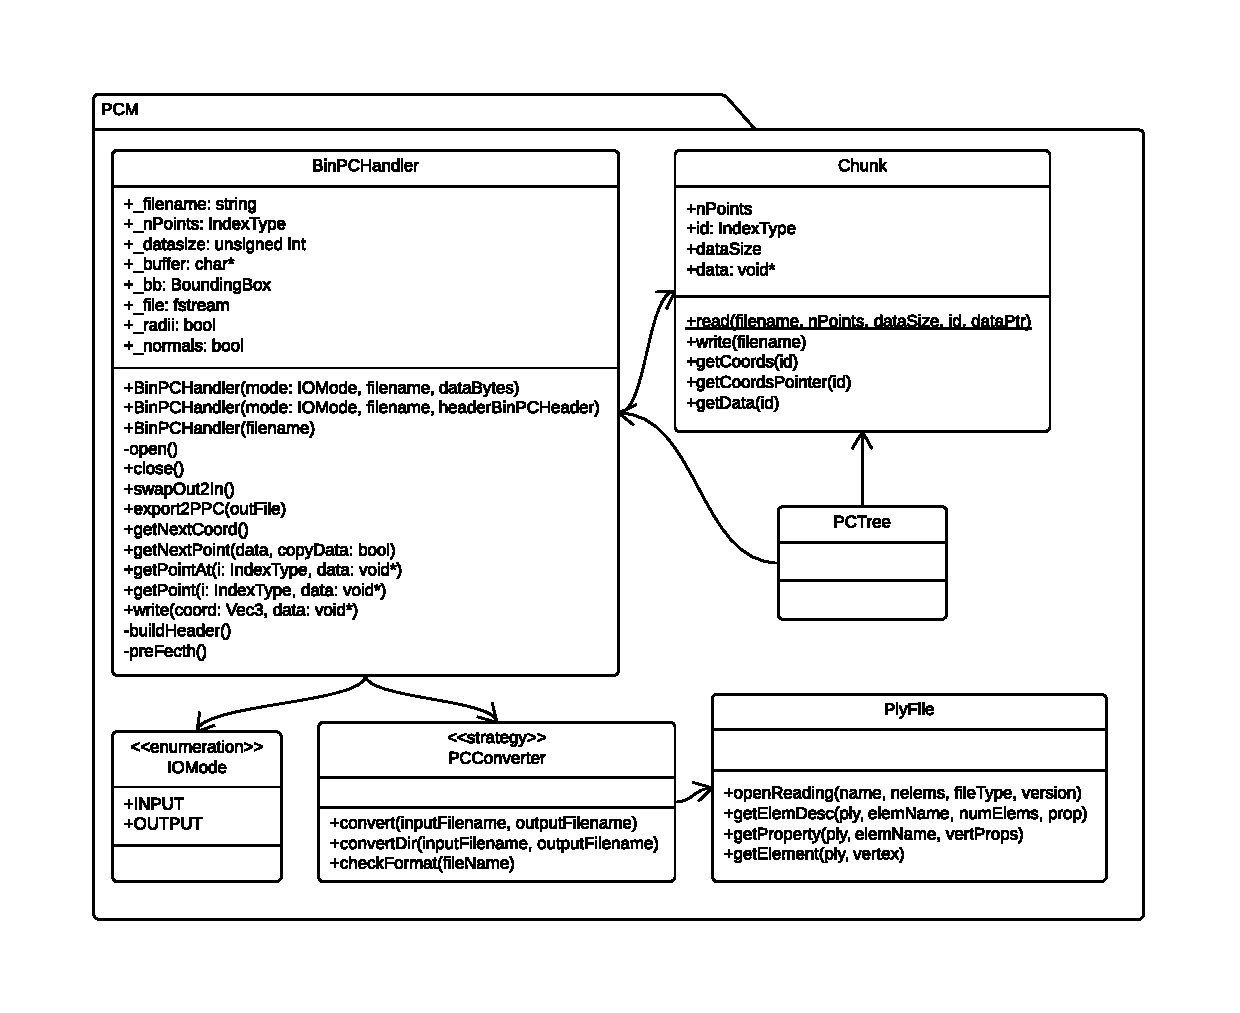
\includegraphics[scale=0.7]{figures/conv_man.pdf}
	\caption[Conversion and management of datasets class diagram]{
		Class diagram of the dataset conversion and management classes.
	}
	\label{conv_man}
\end{figure}

In the diagram in \autoref{conv_man}, the following classes are the most relevant:

\begin{itemize}
	\item \textbf{Chunk:} Minimum unit of data that will be managed by the different cache levels. Its size has to be strictly controlled because of this (no extra information just the basic information necessary to use it). Only has methods to read/write from/to disk.  
	\item \textbf{BinPCHandler:} This class represents the binary format used in the format conversion process and the spatial structure construction. Its objective is to emulate a STL vector, but that resides in disk instead of system memory. This is necessary because during the construction, operations like the calculation of the median will use the whole cloud that will not fit in RAM. With this class, the cloud can be used like if it would fit in primary memory. To improve the performance, it will \textit{pre-fetch} and \textit{buffer} data, after a certain number of requests. It will also allow writing and reading. This class has great performance when accessing data sequentially, but it is not as efficient for random access. 
	\item \textbf{PCConverter:} This will be the class that will provide a single interface to convert any type of point cloud to BPC. The ``strategy'' pattern was used to create this class. It first checks the format of the input point cloud and then delegates the responsibility to the adequate method. It can convert a single file or a set of files stored in a folder.
\end{itemize}

\subsection[Spatial data structure]{Spatial data structure}

The most important class in \autoref{tree_class} is \textbf{PCTree}. The class will encapsulate two of the main functionalities:

\begin{figure}[h]
	\centering
	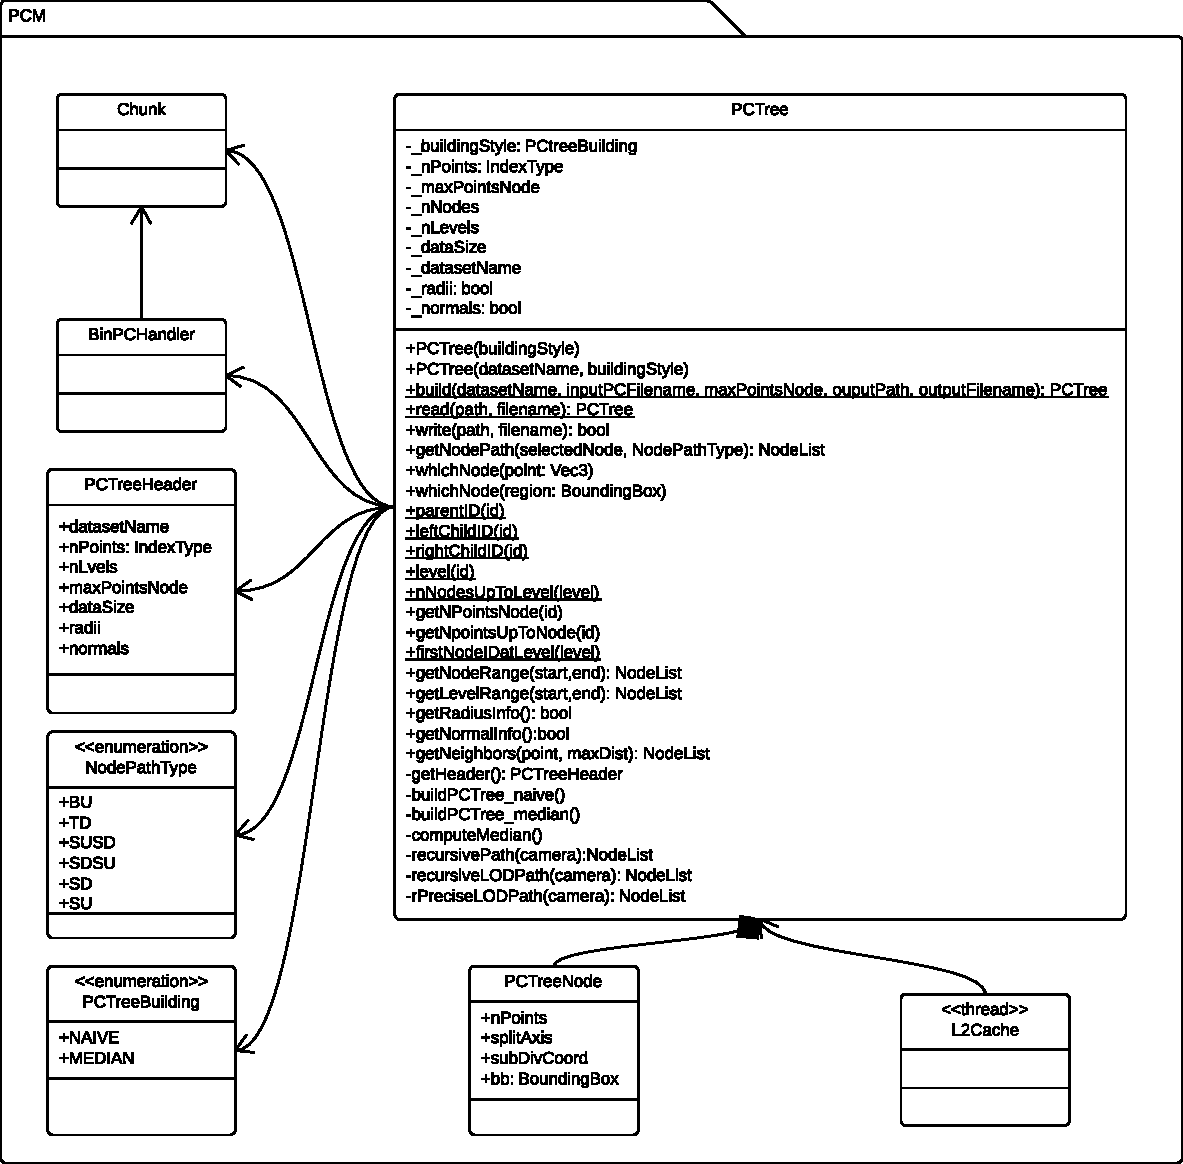
\includegraphics[scale=0.6]{figures/tree_class.pdf}
	\caption[Data strucuture class diagram]{
		Class diagram of the spatial data structure.
	}
	\label{tree_class}
\end{figure}

\begin{itemize}
	\item The construction of the chunk DB and the spatial structure itself. This is done as a pre-process, before using the library. This can be achieved using \textit{PCGen}\footnote{A provided command line utility.} or using the visualizer. 
	\item Managing the multi-resolution tree, obtaining \textit{NodePaths}\footnote{List of nodes to reach a certain area from the tree root.} and performing tree traversals.
\end{itemize}

The tree nodes, represented by the class \textbf{PCTreeNode}, are all kept in a lineal vector for quick access ($O(1)$). There are also some functions valid for any binary tree related to the traversal of the tree; getting the child nodes of a parent, level of a node, etc. There are also functions to read/write the tree from/to disk. Finally, there are also functions to build priority node lists for the visualizer.

TODO assembler log?   

\subsection[Memory hierarchy]{Memory hierarchy}

\begin{figure}[h]
	\centering
	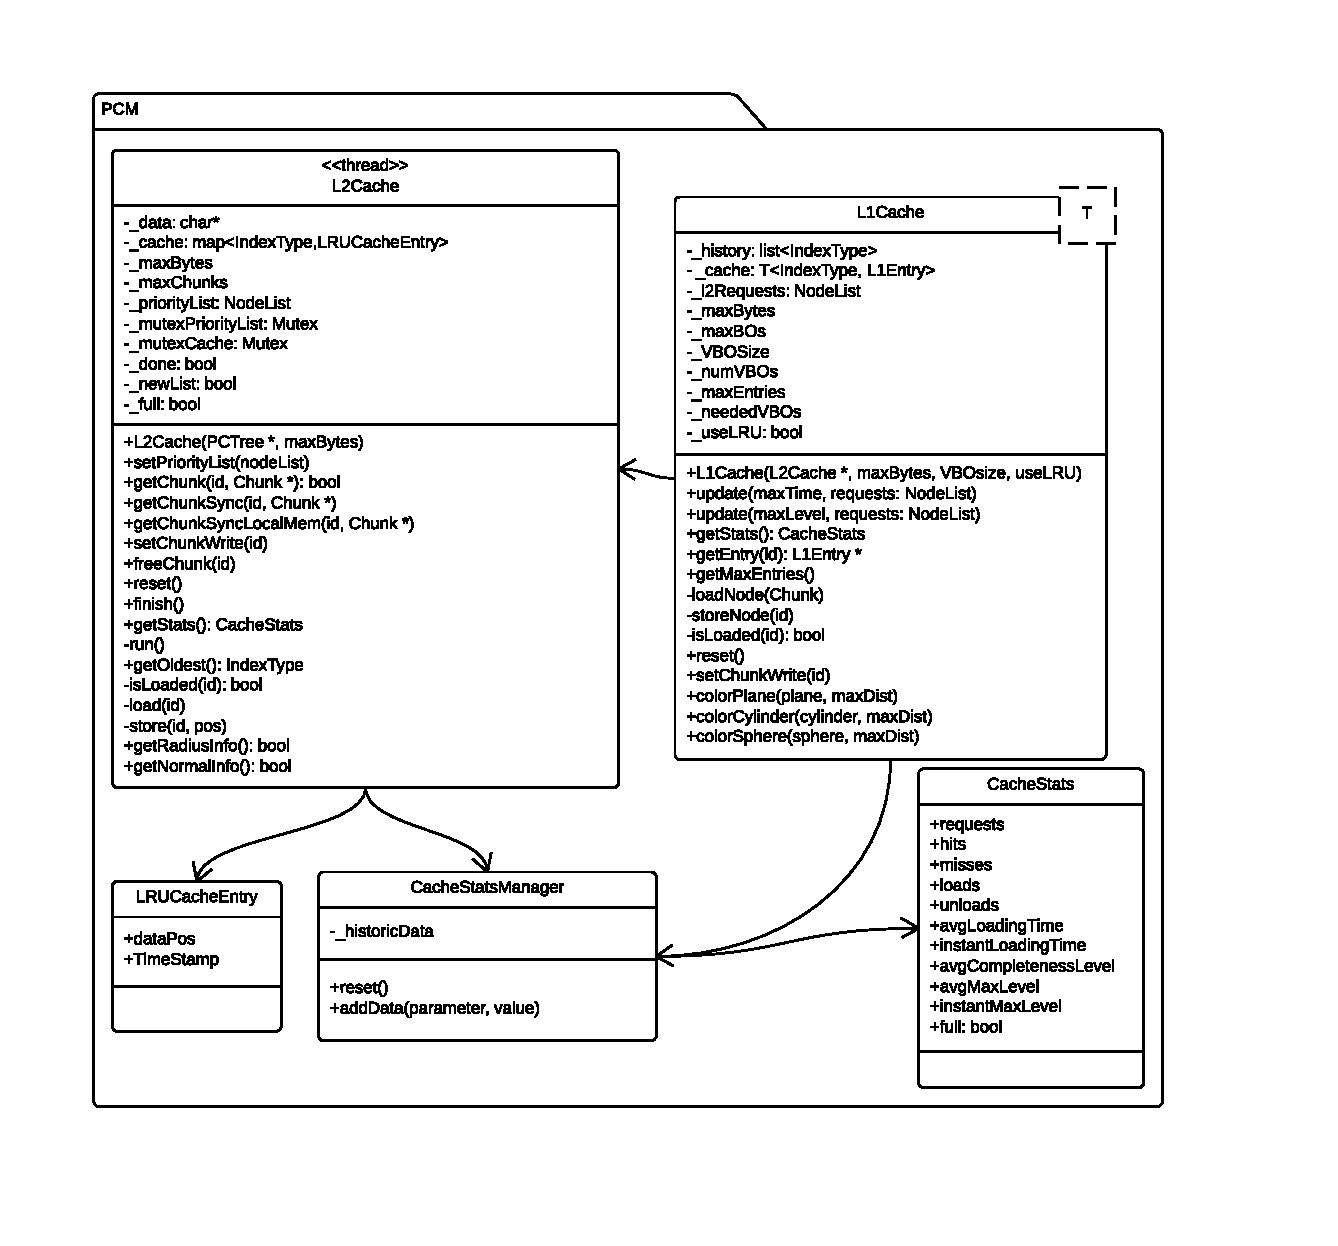
\includegraphics[scale=0.6]{figures/hier_class.pdf}
	\caption[Memory hierarchy class diagram]{
		Class diagram of the memory hierarchy.
	}
	\label{hier_class}
\end{figure}

In \autoref{hier_class} the most significant classes are:

\begin{itemize}
	\item \textbf{L1Cache:} Responsible for loading/storing data in VRAM/RAM and the conversion of chunks in one or multiple VBOs. The class uses a variadic template to let the user choose the type of cache container (\textit{\_cache}). The \textit{update()} method will take care of making the requests to the L2 and the VBO conversion using \textit{load() and store()}.   
	\item \textbf{L2Cache:} Is the class responsible for loading/storing data in RAM/HDD, it inherits from \textbf{Thread} so that it runs on its own thread. As we will mention in \autoref{subsec:L2}, a Map (\textit{\_cache}) keeps references to every chunk that is loaded in the \textit{\_data} attribute. The request list is kept in the attribute \textit{\_priorityList}. Both structures are protected by \textit{Mutex} and a custom \textit{Semaphore}. The \textit{run()} method contains the main loop. 
	\item \textbf{CacheStatsManager:} Both of the previous classes contain an instance of this class. It is in charge of the monitorization of the caches, to get statistics of the cache status. Hits, misses, forced misses, load times, etc.  
\end{itemize}

\subsection[External interface]{External interface}

\begin{figure}[h]
	\centering
	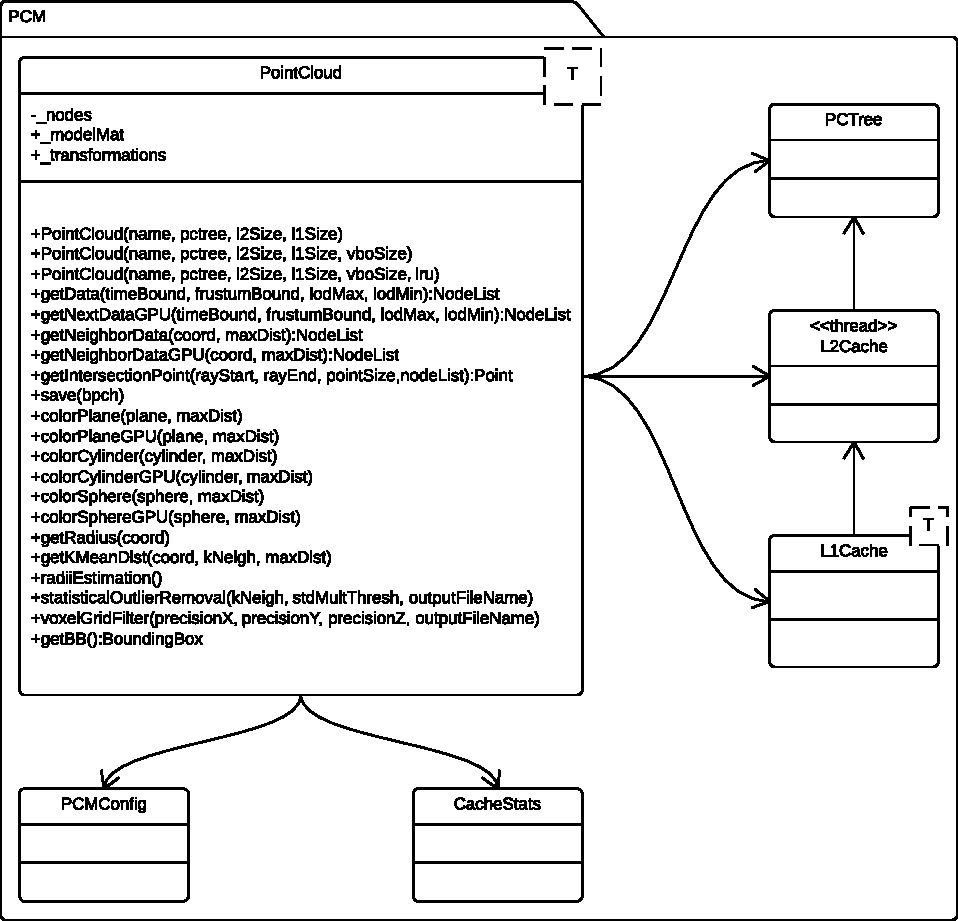
\includegraphics[scale=0.6]{figures/external_interf.pdf}
	\caption[External interface class diagram]{
		Class diagram of the external interface.
	}
	\label{external_interf}
\end{figure}

In \autoref{external_interf} the most important class is \textbf{PointCloud}, this class represents a complete dataset. This class will allow to load or save a dataset, request information about it, request to load an area or access to the spatial structure so that the user can make queries. 

This class is used extensively by the visualizer to simplify the render process. It also provides several point cloud operations, like an statistical outlier removal filter, a voxel filter, radii estimation, etc.

\section[I/O]{Input and output}

This project will support a certain number of common point cloud data input formats. Furthermore, it can also output point cloud or geometric data in certain formats. In this section we will explain all the details related to these two subjects.   

\subsection[Supported point cloud formats]{Supported point cloud formats}

Several new point formats have been added to the capabilities of the point cloud converter utility. PCM will identify automatically the point cloud format and convert it to our own format transparently for the user. 

The supported point cloud input formats are:

\begin{itemize}
	\item \textbf{PTS:} Common ASCII point data format. The first line has the number of points to read, and the rest of the lines all the point data: $(x,y,z) + reflectivity + (R,G,B)$.
	\item \textbf{PTX:} ASCII laser scanning format. The first lines have information about the scan and the number of points scanned. The rest of the lines contain all the point data: $(x,y,z) + reflectivity + (R,G,B)$. 
	\item \textbf{ASC:} Common ASCII point data format in which every line contains information about each point in the cloud: $(x,y,z) + reflectivity + (R,G,B)$.
	\item \textbf{LAS:} Binary laser scanning format, it contains all sorts of information about the scan and the point data that can include: $(x,y,z) + reflectivity + (R,G,B)$.
	\item \textbf{PLY:} PLY is a computer file format known as the Polygon File Format or the Stanford Triangle Format. It can be binary or ASCII, and the project supports both. It contains the following information: $(x,y,z) + (R,G,B) + (n_{x},n_{y},n_{z})$.
	\item \textbf{PCD:} The point cloud format of one of the most used point cloud libraries, \textbf{PCL} \cite{PCL}. As the preceding format, it can be binary or ASCII. Each point can have: $(x,y,z) + (R,G,B)$.   
	\item \textbf{BPC:} Our own binary point cloud data format. It stores information about the cloud and individual points. Each point can have: $(x,y,z) + (R,G,B) + radius + (n_{x},n_{y},n_{z}) + etc$.
\end{itemize}  

Because of the size that this files can reach, they normally are split in several smaller files that range from 500 MB to 1,5 GB. Because of this reason, the ability to read multiple point cloud files in a folder automatically will also be added. 

\subsection[BPC]{Binary Point Cloud}

The point cloud format created for this project (BPC) will now be detailed. It is a binary format that is comprised of a \textbf{header} and the \textbf{point cloud data}. 

The header will contain the following information:

\begin{itemize}
	\item \textbf{Number of points:} The number of points contained in the file.
	\item \textbf{Data size:} Size of the data that accompanies the point (normals, radii, etc.). 
	\item \textbf{Bounding box:} Information of the bounding box that contains the point cloud.
	\item \textbf{Radii:} Indicates if the dataset contains point radii.
	\item \textbf{Normals:} Specifies if the point normals are available.
\end{itemize}  

The rest of the file will contain the point cloud data. The data will be stored contiguously point after point as can be seen in \autoref{chunk} to minimize the file size.

\begin{figure}[h]
	\centering
	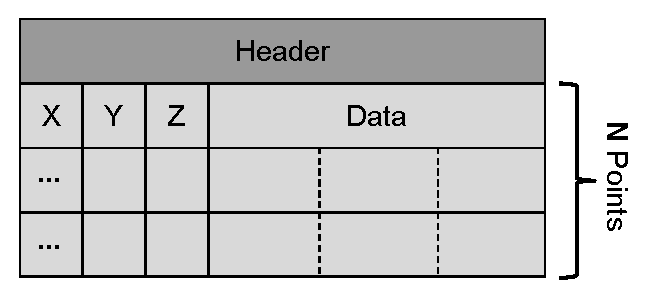
\includegraphics[scale=0.8]{figures/chunk.pdf}
	\caption[Chunk structure]{
		Chunk structure.
	}
	\label{chunk}
\end{figure}

A BPC file is treated like a single chunk that contains the whole cloud, so all of this information is also valid for chunks. A chunk will be the minimum amount of information that the memory hierarchy will deal with. When rendering, the whole cloud will not be stored in a single chunk, since this would not be efficient. Instead, the points in the nodes of the multi-resolution structure will each be stored in a chunk, and the cloud will be an aggregate of all the chunks (see \autoref{chunk_tree}). 

\begin{figure}[h]
	\centering
	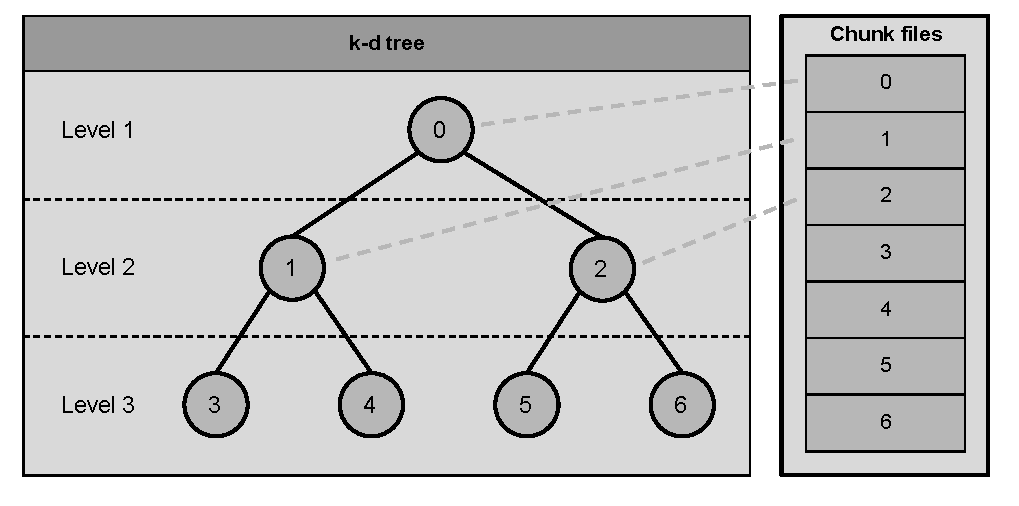
\includegraphics[scale=0.8]{figures/chunk_tree.pdf}
	\caption[Internal tree structure]{
		Internal tree structure. Each node is stored in a chunk file.
	}
	\label{chunk_tree}
\end{figure}

The only big difference between a BPC file and a chunk, is that because the size of a BPC file will be much greater. Therefore it will not be possible to load the complete file at once, and we will rely on an interface class, \textbf{\textcolor{Emerald}{BinPCHandler}}. This interface works in a similar manner to an array in system memory, but accessing permanent memory in an efficient way (this class will be further explained in the \autoref{subsec:conv}). 

\subsection[Output]{Output}

\section[Memory hierarchy]{Memory hierarchy}

One of the principal concepts in PCM is the memory hierarchy management, that is made up of two levels of cache. When it is known that the data that is going to be used is related in some way and the different access types, software caches can yield substantial improvements in the performance of the system. In this case, we work mainly with geometric information obtained from real environments and the cache hierarchy will allow us to exploit the spatial coherence in the data.  

In this project, a cache system with two levels has been implemented. It will take care of the data transfer needs between memory levels (HDD - RAM - VRAM). This system will take into account the spatial relation between the data, and will have an architecture that will not only allow to store datasets in a HDD but anything with a filesystem (e.g. NFS from a network).

\begin{figure}[h]
	\centering
	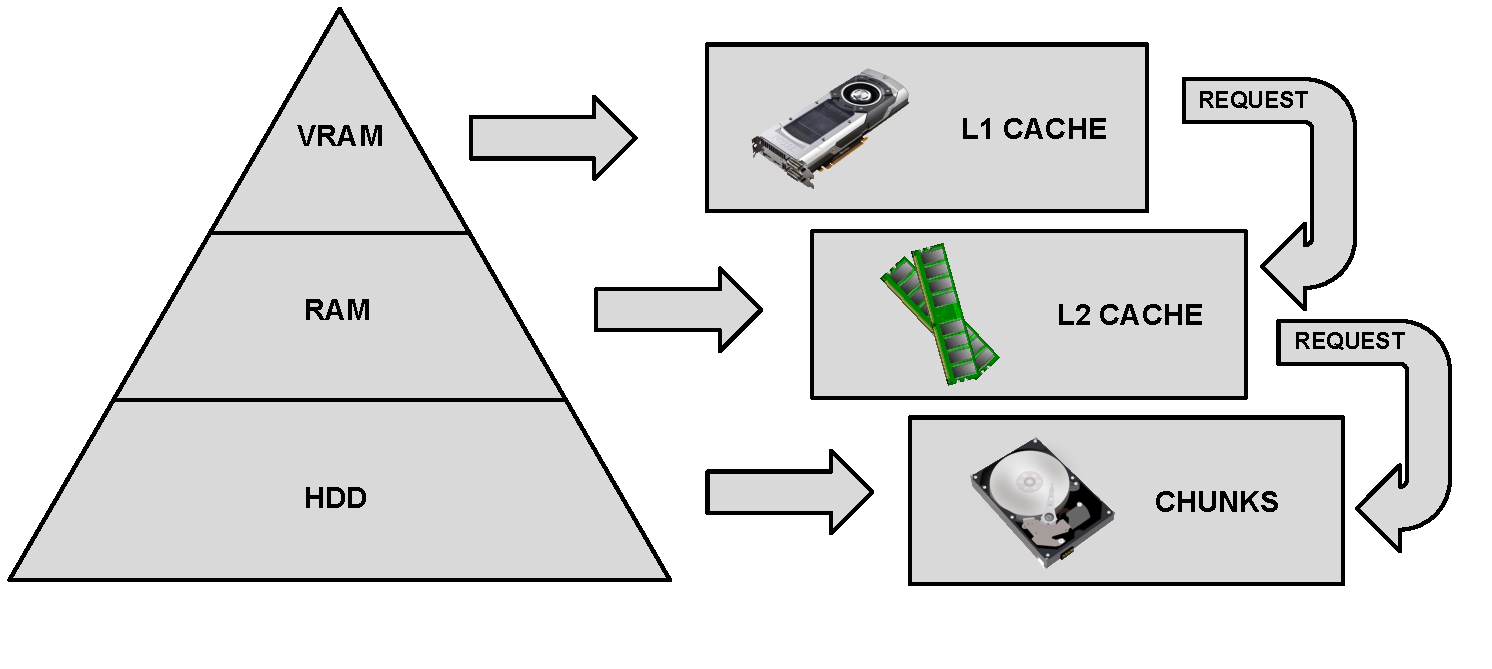
\includegraphics[scale=0.5]{figures/mem_hierch.pdf}
	\caption[Memory hierarchy]{
		Memory hierarchy of PCM.
	}
	\label{mem_hier}
\end{figure}

Between these three levels of memory will circulate the minimum unit of information, the chunk. A chunk is a ``container'' of a data subset, in our case points and data related to them.

The three levels are:

\begin{itemize}
	\item \textbf{Video memory or VRAM:} Volatile memory and less capacity than the next level, but even faster. Only the GPU will use this type of memory. The L1 cache will be created in this memory level.
	\item \textbf{Primary memory or RAM:} Volatile memory and low capacity compared to the next level, but fast. The CPU will use this type of memory. The L2 cache will reside in this cache level. 
	\item \textbf{Secondary memory or HDD:} Persistent memory and high density, but slower than the other two levels. In this level of memory will reside the point database.  
\end{itemize}  

First, in the lowest level, reside the binary files of each chunk. In the next level, RAM memory, a subset of chunks will be stored. Finally in VRAM, the chunks are adapted to a video memory compatible format, so that the GPU can work with them. 

These concepts will be further explained in the next subsections. 

\subsection[L1]{L1 cache}

The first level cache (L1) is in charge of managing the storing and loading of data between primary memory (RAM) and video memory (VRAM). This cache level has been completely reworked, and also has been given the ability to not only load but also store information in primary memory. Even having a similar structure to the L2 cache, because of the characteristics of GPU processes, its operation is synchronous. 

Its biggest responsibility, apart from the corresponding memory hierarchy management, will be the conversion of chunks of data to \textit{VBOs}\footnote{\textit{Vertex Buffer Object}: Structure that allows to store arrays of data in video memory.} in VRAM and viceversa. A chunk may have to be broken up into several VBOs depending on its size, so that optimal sizes of VBOs can be maintained for the GPU.

\begin{figure}[h]
	\centering
	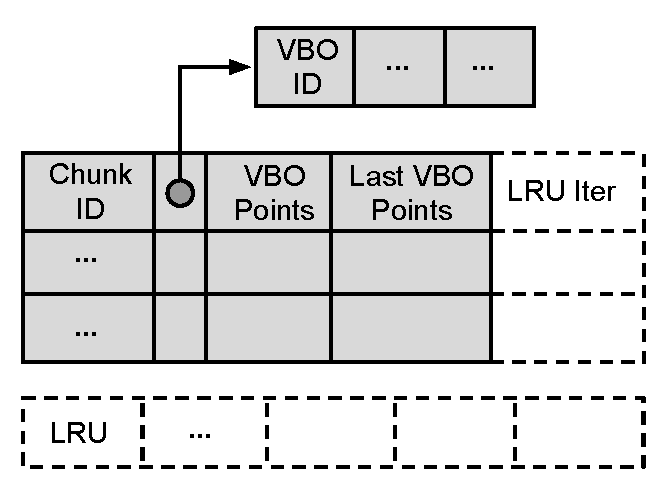
\includegraphics[scale=0.7]{figures/l1_cache.pdf}
	\caption[L1 cache structure]{
		L1 cache structure.
	}
	\label{l1_cache}
\end{figure}

The following list will explain each of the fields that make up the cache structure (see \autoref{l1_cache}):

\begin{itemize}
	\item \textbf{Chunk ID:} Id of the chunk stored in L1 cache.
	\item \textbf{VBO ID:} IDs of the VBOs used to store points in the L1 cache entry.
	\item \textbf{VBO Points:} Number of points stored in all but the last VBO in the cache entry.
	\item \textbf{Last VBO Points:} Number of points in the last VBO in the cache entry.
	\item \textbf{LRU Iter:} Iterator to cache entry in LRU access record for fast updating of LRU.
	\item \textbf{LRU:} Least Recently Used chunk. 
	\item \textbf{Write:} Flag that marks chunk for storing. 
\end{itemize} 

Also two replacement policies were implemented:

\begin{itemize}
	\item \textbf{Naive:} Erase any data block that is not necessary looping over the complete cache one time. This method does not take into account when was the last time that a block was last used, if it is not necessary it will be erased. 
	\item \textbf{LRU\footnote{\textit{Least Recently Used}}:} This algorithm, will replace the elements that have been used least recently if the cache is full. If not full it will keep inserting nodes until it is.  
\end{itemize} 

To store the list of nodes currently in the cache two STL\footnote{\textit{Standard Template Library}} data structures can be used:

\begin{itemize}
	\item \textbf{Map:} An associative container with key-value pairs with ordered unique keys. Complexity of searches and element access is logarithmic in size: $O(\log n)$. 
	\item \textbf{HashMap:} It also contains key-value pairs with unique keys but without an order, element access is done using a hash function. Complexity of searches and element access is constant in the average case: $O(1)$ and linear in size in the worst case: $O(n)$.
\end{itemize}

Either of these two structures will meet our objective of making cache searches fast, as this is a crucial function that will be frequently used. Theoretically the use of one or the other depends on the number of nodes that the cache will contain. A Map will be faster with less elements, while the HashMap will be faster with big quantities of nodes. 

Another implemented feature are types of cache requests, there are several available:

\begin{itemize}
	\item \textbf{Restricted by time:} In order for the render process to be interactive and that no freezes occur, we will limit loading of VBOs by time. This type of petition will be limited by the time that the user desires (e.g. 3 ms). The cache will load as much nodes as possible in the given time and if the maximum time is reached it will stop loading nodes, even if there are still nodes missing. 
	\item \textbf{Restricted by level:} This type of request is usually used in GPGPU calculations, where no interactivity is needed. The user will specify a level of precision and the cache will load as many nodes as necessary for that level of detail.
\end{itemize}

This cache not only can read and load nodes from L2, it also has the ability to store changes made in video memory (L1) in RAM (L2). The user can choose if he wants the changes made in GPU (e.g. an OpenCL kernel) to be persistent or not.

When the node is evicted from the cache, its changes will be written to the L2 cache prior to its deletion. In the \autoref{l1_write} we not only show how to write changes to other cache levels, but also how to use PCM with its new \textbf{\textcolor{Emerald}{PointCloud}} interface to loop over the complete cloud out of core and perform some custom operation.

This process is completely transparent for the user, that will only have to use this example code:
\\
\lstset{language=C++,frame=shadowbox,rulesepcolor=\color[gray]{0.8},lineskip=10pt, 
		keywordstyle=\color{VioletRed}\bfseries,
		emph={PointCloud}, emphstyle=\color{Emerald}\bfseries,
		emph={[2]setChunkWriteL1,getNextDataGPU,getL1Entry,makeChangesGPU}, emphstyle={[2]\color{PineGreen}}}
\begin{lstlisting}[caption={How to write data to L1 chunk.},captionpos=b,label={l1_write}]
 PointCloud cloud(...);

 while (cloud.getNextDataGPU(list)) {
 	for (auto& node:list) {		
		auto * VBOdata = cloud.getL1Entry(node);
		if (VBOdata) {
			makeChangesGPU(node);
			cloud.setChunkWriteL1(node);
		}		
	}
 }
\end{lstlisting}

\subsection[L2]{L2 cache}
\label{subsec:L2}

The second level cache L2, will be in charge of transferring data (chunks) from disk to system memory (RAM). The replacement policy used in this cache is LRU \cite{taibo} as this is the most adequate policy for these types of systems. 

To better use the resources available nowadays (multi-core CPUs), this cache will run on its own thread. Also since the massive datasets that we will deal with require a lot of computational power for even the simplest operations, this cache will be prepared to deal with simultaneous requests from different work threads. All of this is achieved with careful use of \textit{mutex}\footnote{A synchronization mechanism for enforcing limits on access to a resource in an environment where there are many threads of execution.} and \textit{semaphores}\footnote{A variable or abstract data type that is used for controlling access, by multiple processes, to a common resource in a parallel programming or a multi user environment.}. 

\begin{figure}[h]
	\centering
	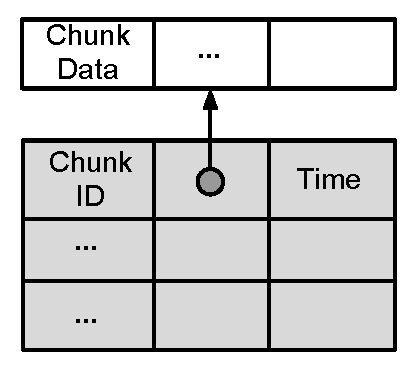
\includegraphics[scale=0.9]{figures/L2.pdf}
	\caption[L2 structure]{
		L2 cache structure.
	}
	\label{l2_structure}
\end{figure}

The following list will explain each of the cache structure fields (see \autoref{l2_structure}):

\begin{itemize}
	\item \textbf{Chunk ID:} Id of the chunk stored in L2 cache.
	\item \textbf{Position:} Position of the chunk in the structure that contains all of them.
	\item \textbf{Time:} Time in which the node was last accessed.
\end{itemize} 

Next, the responsibilities of the L2 cache are:

\begin{itemize}
	\item Load petition lists from disk that are requested by the upper cache level (L1).
	\item Keep a ``repository'' of recently loaded chunks, that because of the nature of the spatial structure, will be utilized again with a high probability. 
	\item Ask the spatial structure which files correspond to the requested nodes.
	\item Keep memory coherence of the system, with a Map that matches node IDs with their corresponding chunk in memory. 
	\item If the user desires it, write changes to disk.   
\end{itemize} 

The main loop can be summed up in the following actions. First, it waits until a new petition arrives, when it does, it loads the requested nodes in order. If during the loading of the list a new one appears, the old one is discarded and the process begins again.

This cache can work in one of two ways:

\begin{itemize}
	\item \textbf{Synchronous:} A node is requested and loaded immediately. 
	\item \textbf{Asynchronous:} A list of nodes is requested and they are loaded in order as soon as possible.
\end{itemize}

This cache is capable of not only reading data from the HDD, but also writing modified data from RAM to disk. This is achieved in a similar fashion to the L1. A complete loop over the whole cloud to perform an operation using the CPU and then writing it to disk, can be seen in \autoref{l2_write}.
\\
\lstset{emph={PointCloud,Chunk}, emphstyle=\color{Emerald}\bfseries,
		emph={[2]setChunkWriteL2,getNextData,getChunkL2,makeChanges,freeChunkL2}, emphstyle={[2]\color{PineGreen}}}
\begin{lstlisting}[caption={How to perform an operation using the L2 and store the changes.},captionpos=b,label={l2_write}]
 PointCloud cloud(...);

 while (cloud.getNextData(list)) {
 	for (auto& node:list) {		
		Chunk chunk;
		cloud.getChunkL2(node, chunk);
		makeChanges(chunk);
		cloud.setChunkWriteL2(node);	
		cloud.freeChunkL2(node);	
	}
 }
\end{lstlisting}

The cache hit rate will be really high, because of the topology of the spatial structure. If an algorithm needs to reach the maximum level of detail in different zones, because the levels are additive, it will have to add up all the information contained in the node path from the root to the leaf. But in regions of space that are close, that means they will share a lot of nodes (see \autoref{node_sharing}). 

\begin{figure}[h]
	\centering
	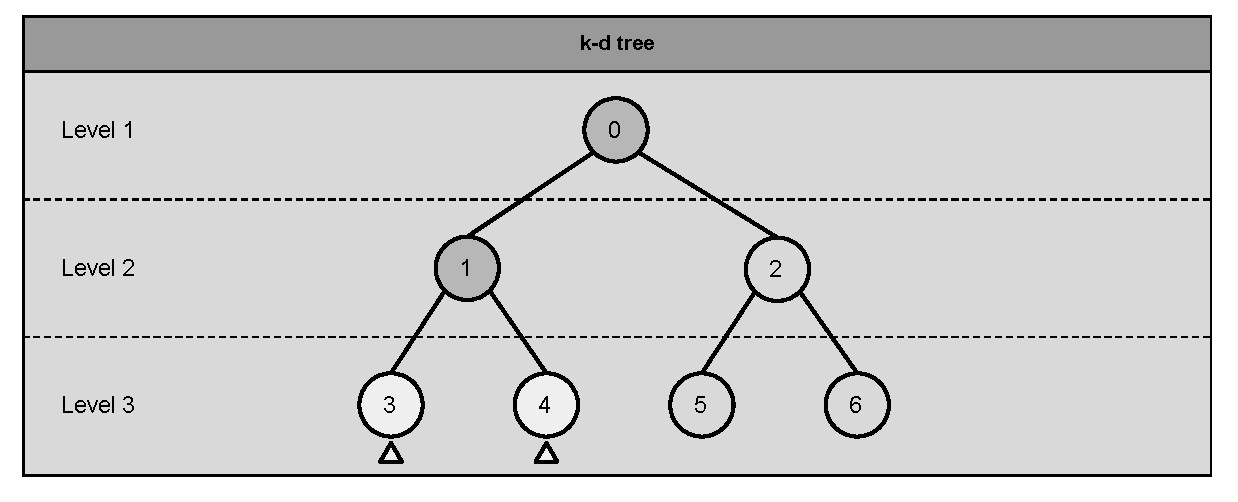
\includegraphics[scale=0.6]{figures/node_sharing.pdf}
	\caption[Common nodes close paths]{
		Two node paths spatially close (3 and 4), in order to reach the maximum level of detail (level 2) share nodes 0 and 1.
	}
	\label{node_sharing}
\end{figure}

\subsection[PCM Benchmark]{PCM Benchmark}

Since we wanted to have a quick and convenient way to test PCM, we created this utility in \textit{Python} to achieve this purpose. PCMBenchmark is a Python benchmark suite that automatically tests PCM and outputs the corresponding metrics for the user to see or use. 

In order for PCMBenchmark to work it uses a certain directory structure:

\begin{itemize}
	\item \textbf{bin:} With \textbf{debug} and \textbf{release} sub-directories that contain the corresponding PCM executables (user creation required).
	\item \textbf{dataset:} Contains the test dataset (user creation required).
	\item \textbf{data:} Automatically created directory that contains testing data. This is raw data just in case the user will want to process the data on its own.
	\item \textbf{trees:} Automatically created directory that contains automatically generated k-d trees.
\end{itemize} 

\begin{figure}[h]
	\centering
	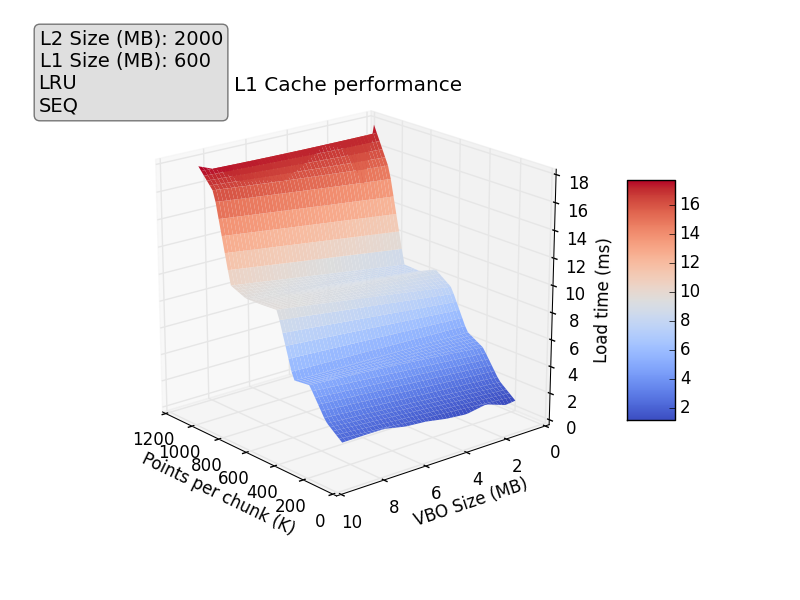
\includegraphics[scale=0.7]{figures/benchmark.png}
	\caption[Sample PCMBenchmark output]{
		A sample output graph created by the benchmark suite.
	}
	\label{benchmark}
\end{figure}

Once the user has the directory structure created, its just a matter of copying and pasting to test PCM in different machines. The process will be completely transparent for the user that will only need to check the resulting graphs (see \autoref{benchmark}).

The outputs that the benchmark suite creates are:

\begin{itemize}
	\item \textbf{Graphs:} Available in the root directory as a series of .png files. This is the most user friendly output of the tool, a series of graphs that show the metrics in a graphical sense.
	\item \textbf{System information:} Stored in a text file called \textit{sys\_info.txt} that contains common system info.
	\item \textbf{Raw data:} Automatically generated data to create the graphs. Suitable for further processing by an advanced user.
\end{itemize} 

The only system requirements are:

\begin{itemize}
	\item \textbf{Python 3.3}
	\item \textbf{MatPlotLib}
	\item \textbf{NumPy}
\end{itemize} 

With this tool the testing in multi-platform environments is greatly simplified.

\section[Results]{Results}

Two computers with different hardware where used for testing. The first, \textbf{Computer 1} has the following specs:

\begin{itemize}
	\item Intel Core i7-3770 CPU (4 cores, 8 threads)
	\item NVIDIA GT 640 graphics card
	\item 16 GB of 1600 MHz DDR3 RAM
	\item WDC WD10EZRX HDD
\end{itemize} 

The second, \textbf{Computer 2} has the following specifications:

\begin{itemize}
	\item Intel Core i7-4930K CPU (6 cores, 12 threads)
	\item NVIDIA GTX 780Ti graphics card
	\item 16 GB of 2133 MHz DDR3 RAM
	\item WD Caviar Black HDD
\end{itemize} 

The operating system used to run the tests was Windows 7 x64, with VC{}\verb!++! v110 compiler. The libraries used were:

\begin{itemize}
	\item OSG 3.0.1
	\item Freeglut 2.8.1
	\item GLEW 1.10.0
	\item PCL 1.7.1
\end{itemize} 

The datasets that will be used for testing are described in \autoref{dataset_table}.

\begin{table}
\begin{center}
\begin{tabular}{cccc}
\toprule
Image & Name & Points & Features \\
\midrule
 \raisebox{-.5\height}{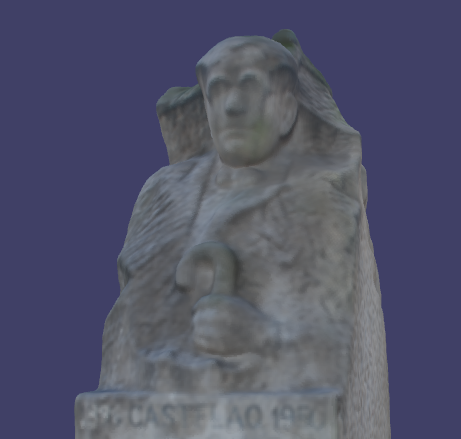
\includegraphics[scale=0.13]{figures/castelao.png}} & Castelao & $\sim 500K$  & Color, Normals \\[1cm]
 \raisebox{-.5\height}{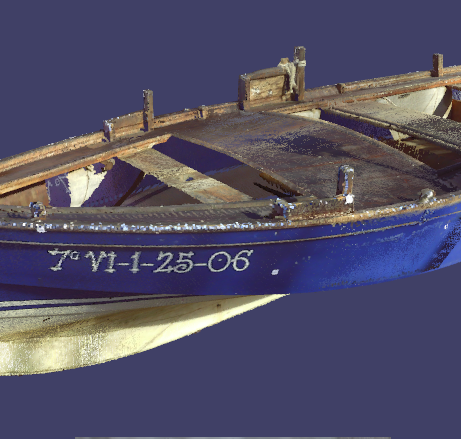
\includegraphics[scale=0.13]{figures/dorna.png}} & Dorna & $\sim 3M$  & Color \\[1cm]
 \raisebox{-.5\height}{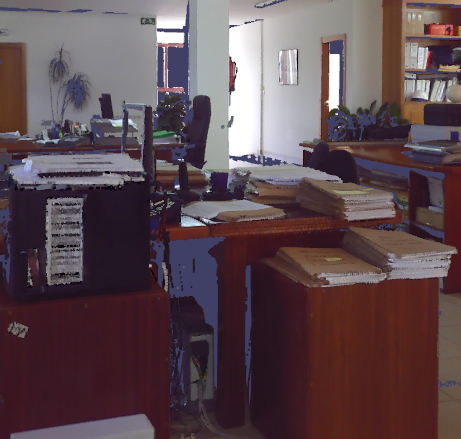
\includegraphics[scale=0.13]{figures/oficina.png}} & Oficina & $\sim 30M$  & Color \\[1cm]
 \raisebox{-.5\height}{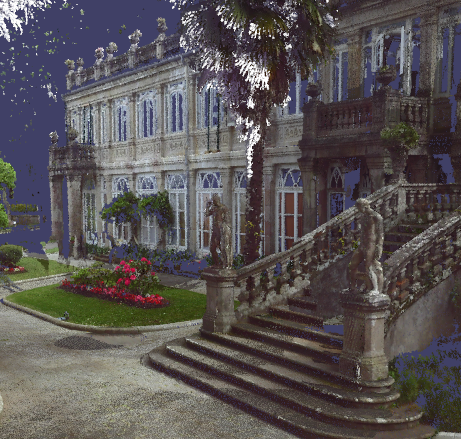
\includegraphics[scale=0.13]{figures/lourizan.png}} & Lourizan & $\sim 90M$  & Color \\[1cm]
 \raisebox{-.5\height}{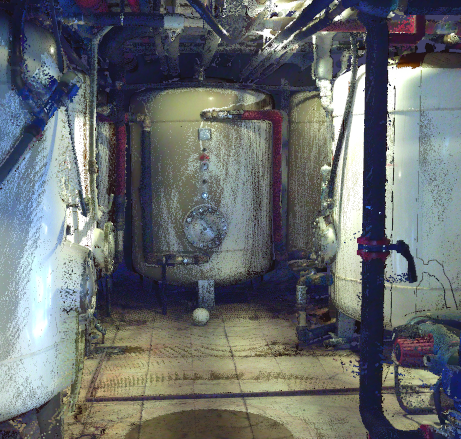
\includegraphics[scale=0.13]{figures/CALD.png}} & CALD & $\sim 200M$  & Color \\[1cm]
 \raisebox{-.5\height}{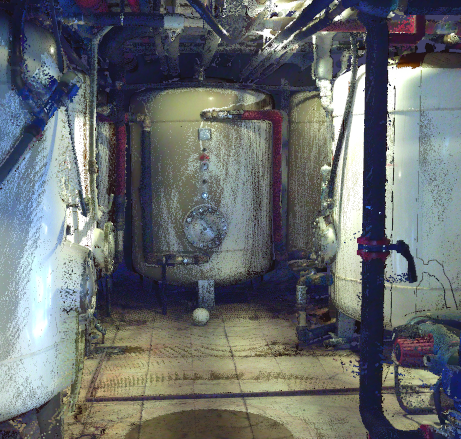
\includegraphics[scale=0.13]{figures/CALD.png}} & Baron & $\sim 500M$  & Color \\[1cm]
 \raisebox{-.5\height}{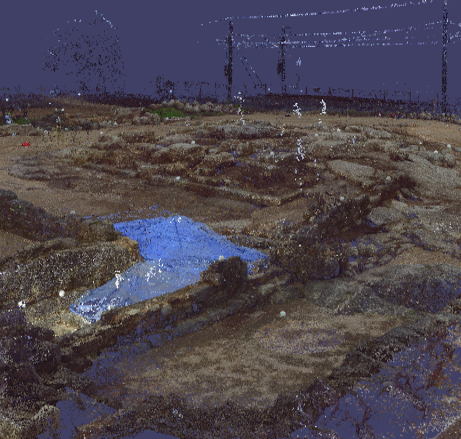
\includegraphics[scale=0.13]{figures/castelo.png}} & Castelo & $\sim 1000M$  & Color \\
\bottomrule
\end{tabular}
\end{center}
\caption[Tested datasets]{
		Table showing the datasets that were used when testing.
}
\label{dataset_table}
\end{table}

In the first test (see \autoref{radii_est_castelao}), we will estimate the radii using the CPU (using all threads available) and GPU. We can observe that as the chunk size decreases, the estimation is faster. This is because there are less intersection tests to be performed, since a lot of nodes can be discarded as they will not belong to the neighborhood of each point. 

It is also interesting to highlight the fact that the GPU is slower than the CPU, this happens due to the setup of the OpenCL kernel. The transfering of information from RAM to VRAM and the kernel setup calls outweigh the benefits of the GPGPU implementation. This means, that the computation of the radii in GPU is faster, but when dealing with a relatively cheap operation like the former, the setup of the kernel takes too much time compared to the kernel execution time and makes the GPU lose against the CPU. 

\begin{figure}[h]
	\centering
	\subfigure[Computer 1]{\label{fig:a}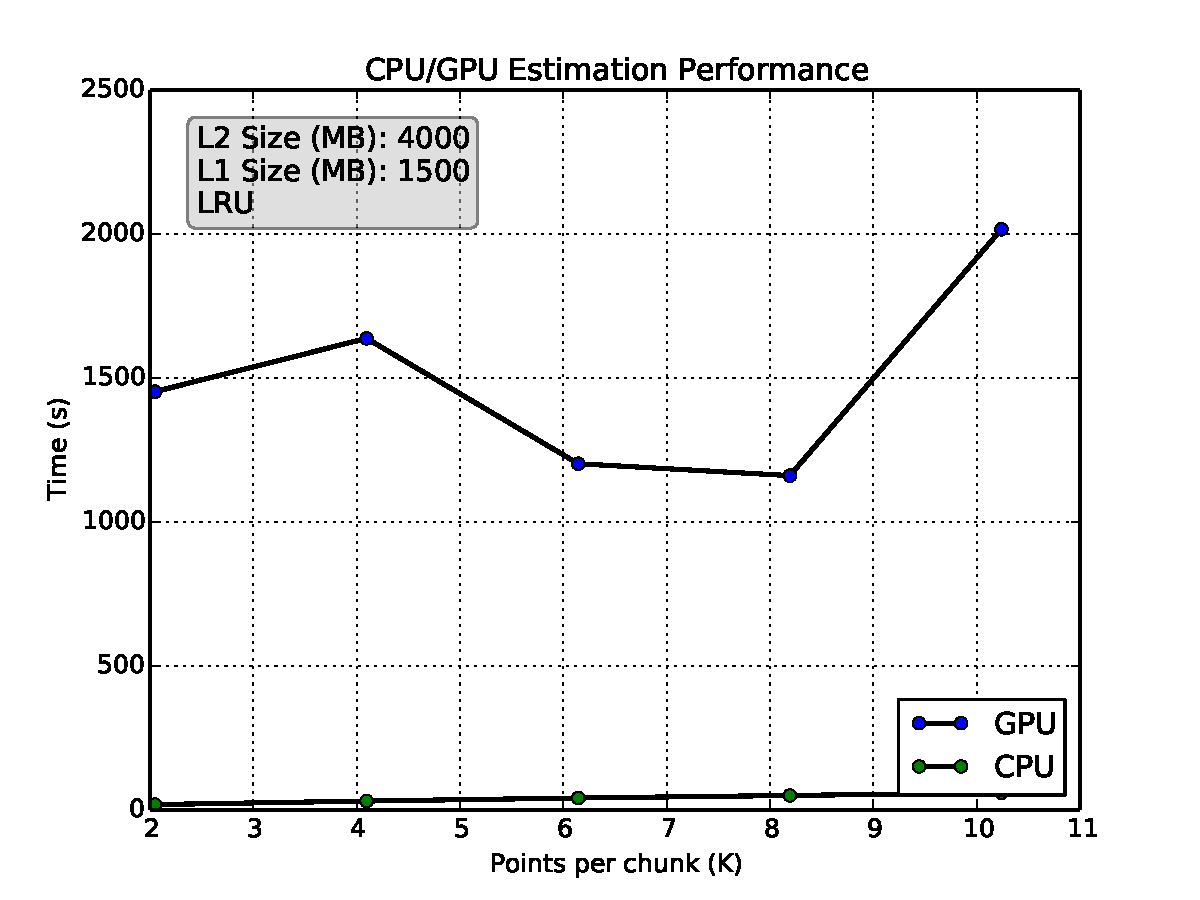
\includegraphics[width=0.49\textwidth]{figures/cpu_gpu_est_cast_640.pdf}}
	\subfigure[Computer 2]{\label{fig:b}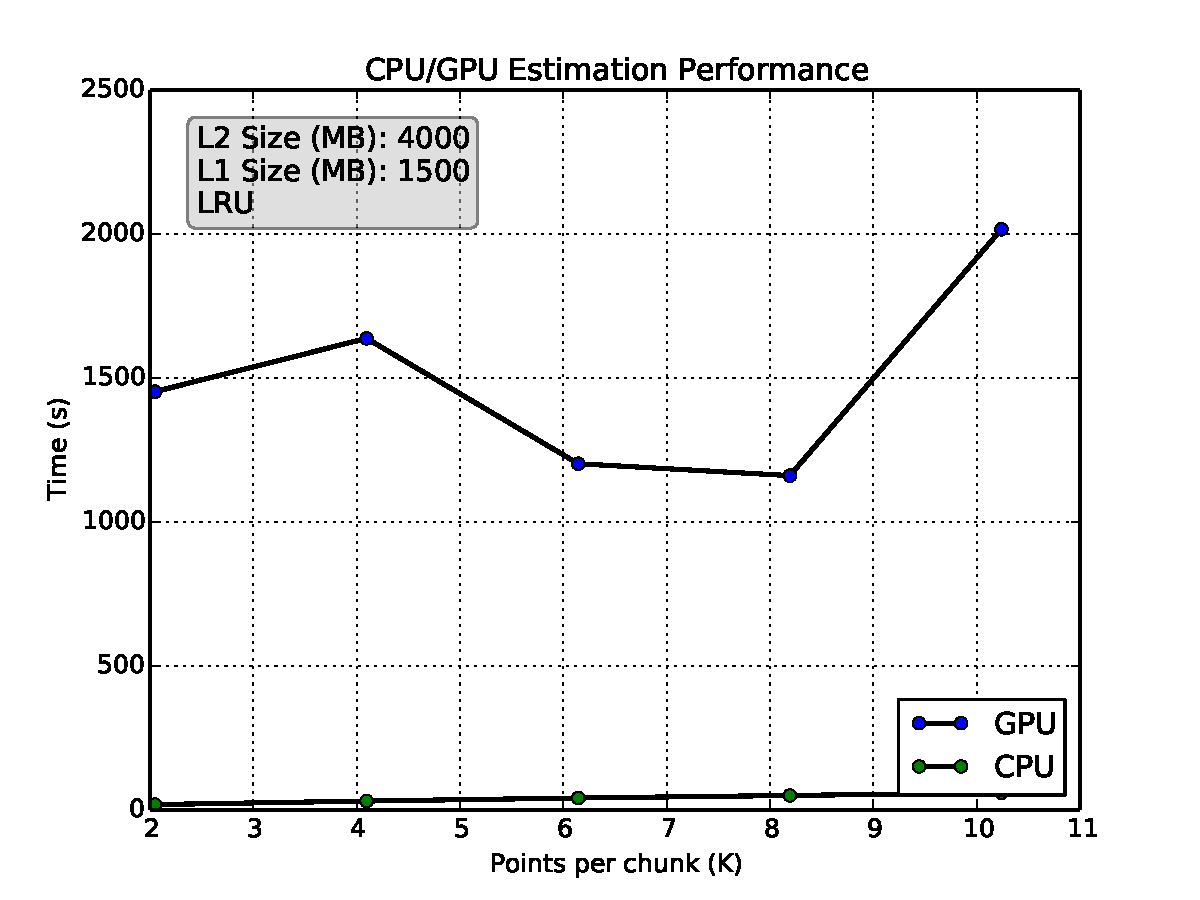
\includegraphics[width=0.49\textwidth]{figures/cpu_gpu_est_cast_640.pdf}}
	\caption[CPU/GPU radii estimation Castelao]{
		Graphs showing the estimation times in the Castelao dataset.
	}
	\label{radii_est_castelao}
\end{figure}

The next test also compares the radii estimation times in the two test machines, but this time with the Dorna dataset (see \autoref{radii_est_dorna}).

\begin{figure}[h]
	\centering
	\subfigure[Computer 1]{\label{fig:a}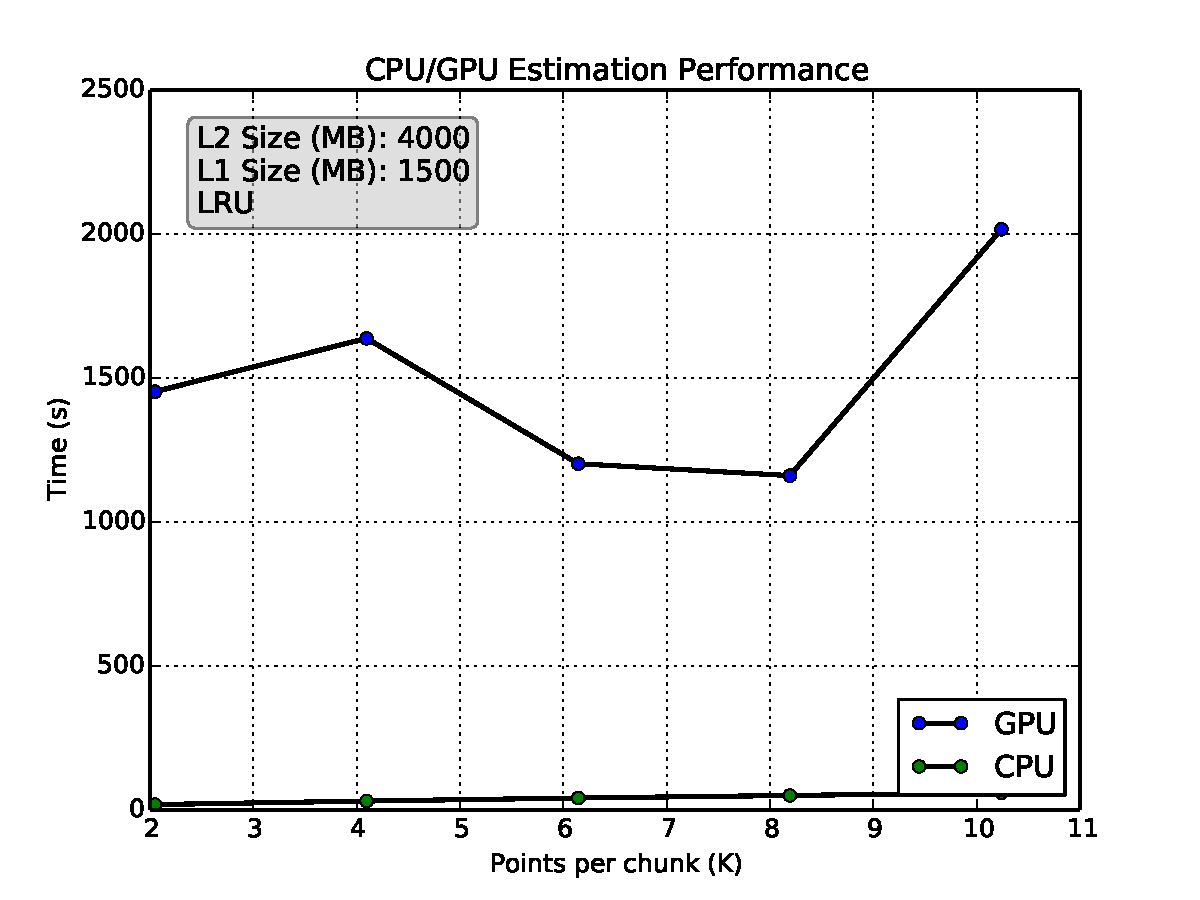
\includegraphics[width=0.49\textwidth]{figures/cpu_gpu_est_cast_640.pdf}}
	\subfigure[Computer 2]{\label{fig:b}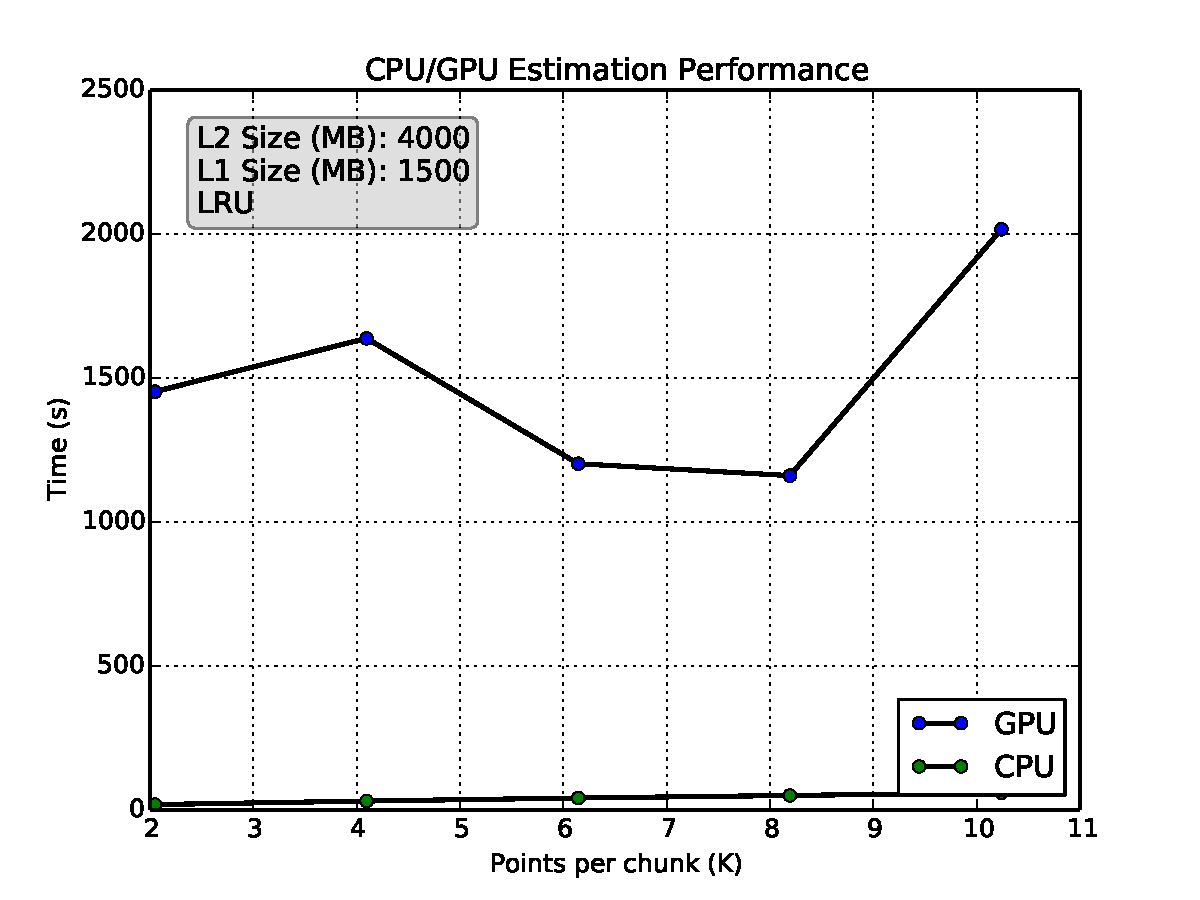
\includegraphics[width=0.49\textwidth]{figures/cpu_gpu_est_cast_640.pdf}}
	\caption[CPU/GPU radii estimation Dorna]{
		Graphs showing the estimation times in the Dorna dataset.
	}
	\label{radii_est_dorna}
\end{figure}
